Before describing \PNAME's DRAM timing-models~(Section~\ref{sec:dram-timing-model}), we review some relevant background
on DRAM memory systems.

\section{DRAM Device Architecture}\label{sec:dram-arch}
In a DRAM IC, arrays of bit cells are hierarchically arranged into multiple
parallel \textit{banks}. Banks provide the primitive level of concurrency in a
DRAM memory system: they can service independent requests assuming they do not
simultaneously require shared resources like the data, address and command
buses.  Multiple DRAM ICs can be arranged in parallel to widen the data bus;
address and command buses fan out to each IC.

A basic DRAM operation requires a series of three commands: \textit{activate (ACT)},
\textit{column access (CAS)}, and \textit{precharge (PRE)}. The ACT command
enables the word-lines of the array corresponding to a single \textit{row} of
the bank. The cells of the row are sensed and saved in a \textit{row
buffer}. A CAS command then selects a subset of the row buffer to
read or write; data is bursted over successive clock edges. While the row
buffer remains \textit{open}, the row can be accessed by issuing new CAS
commands. To access a different row, a PRE command must be
issued to \textit{close} the row and recharge the bit-lines.
%The organization of a typical DRAM device is shown in Figure~\ref{fig:dram-device}.

%\begin{figure}
%	\centering
%	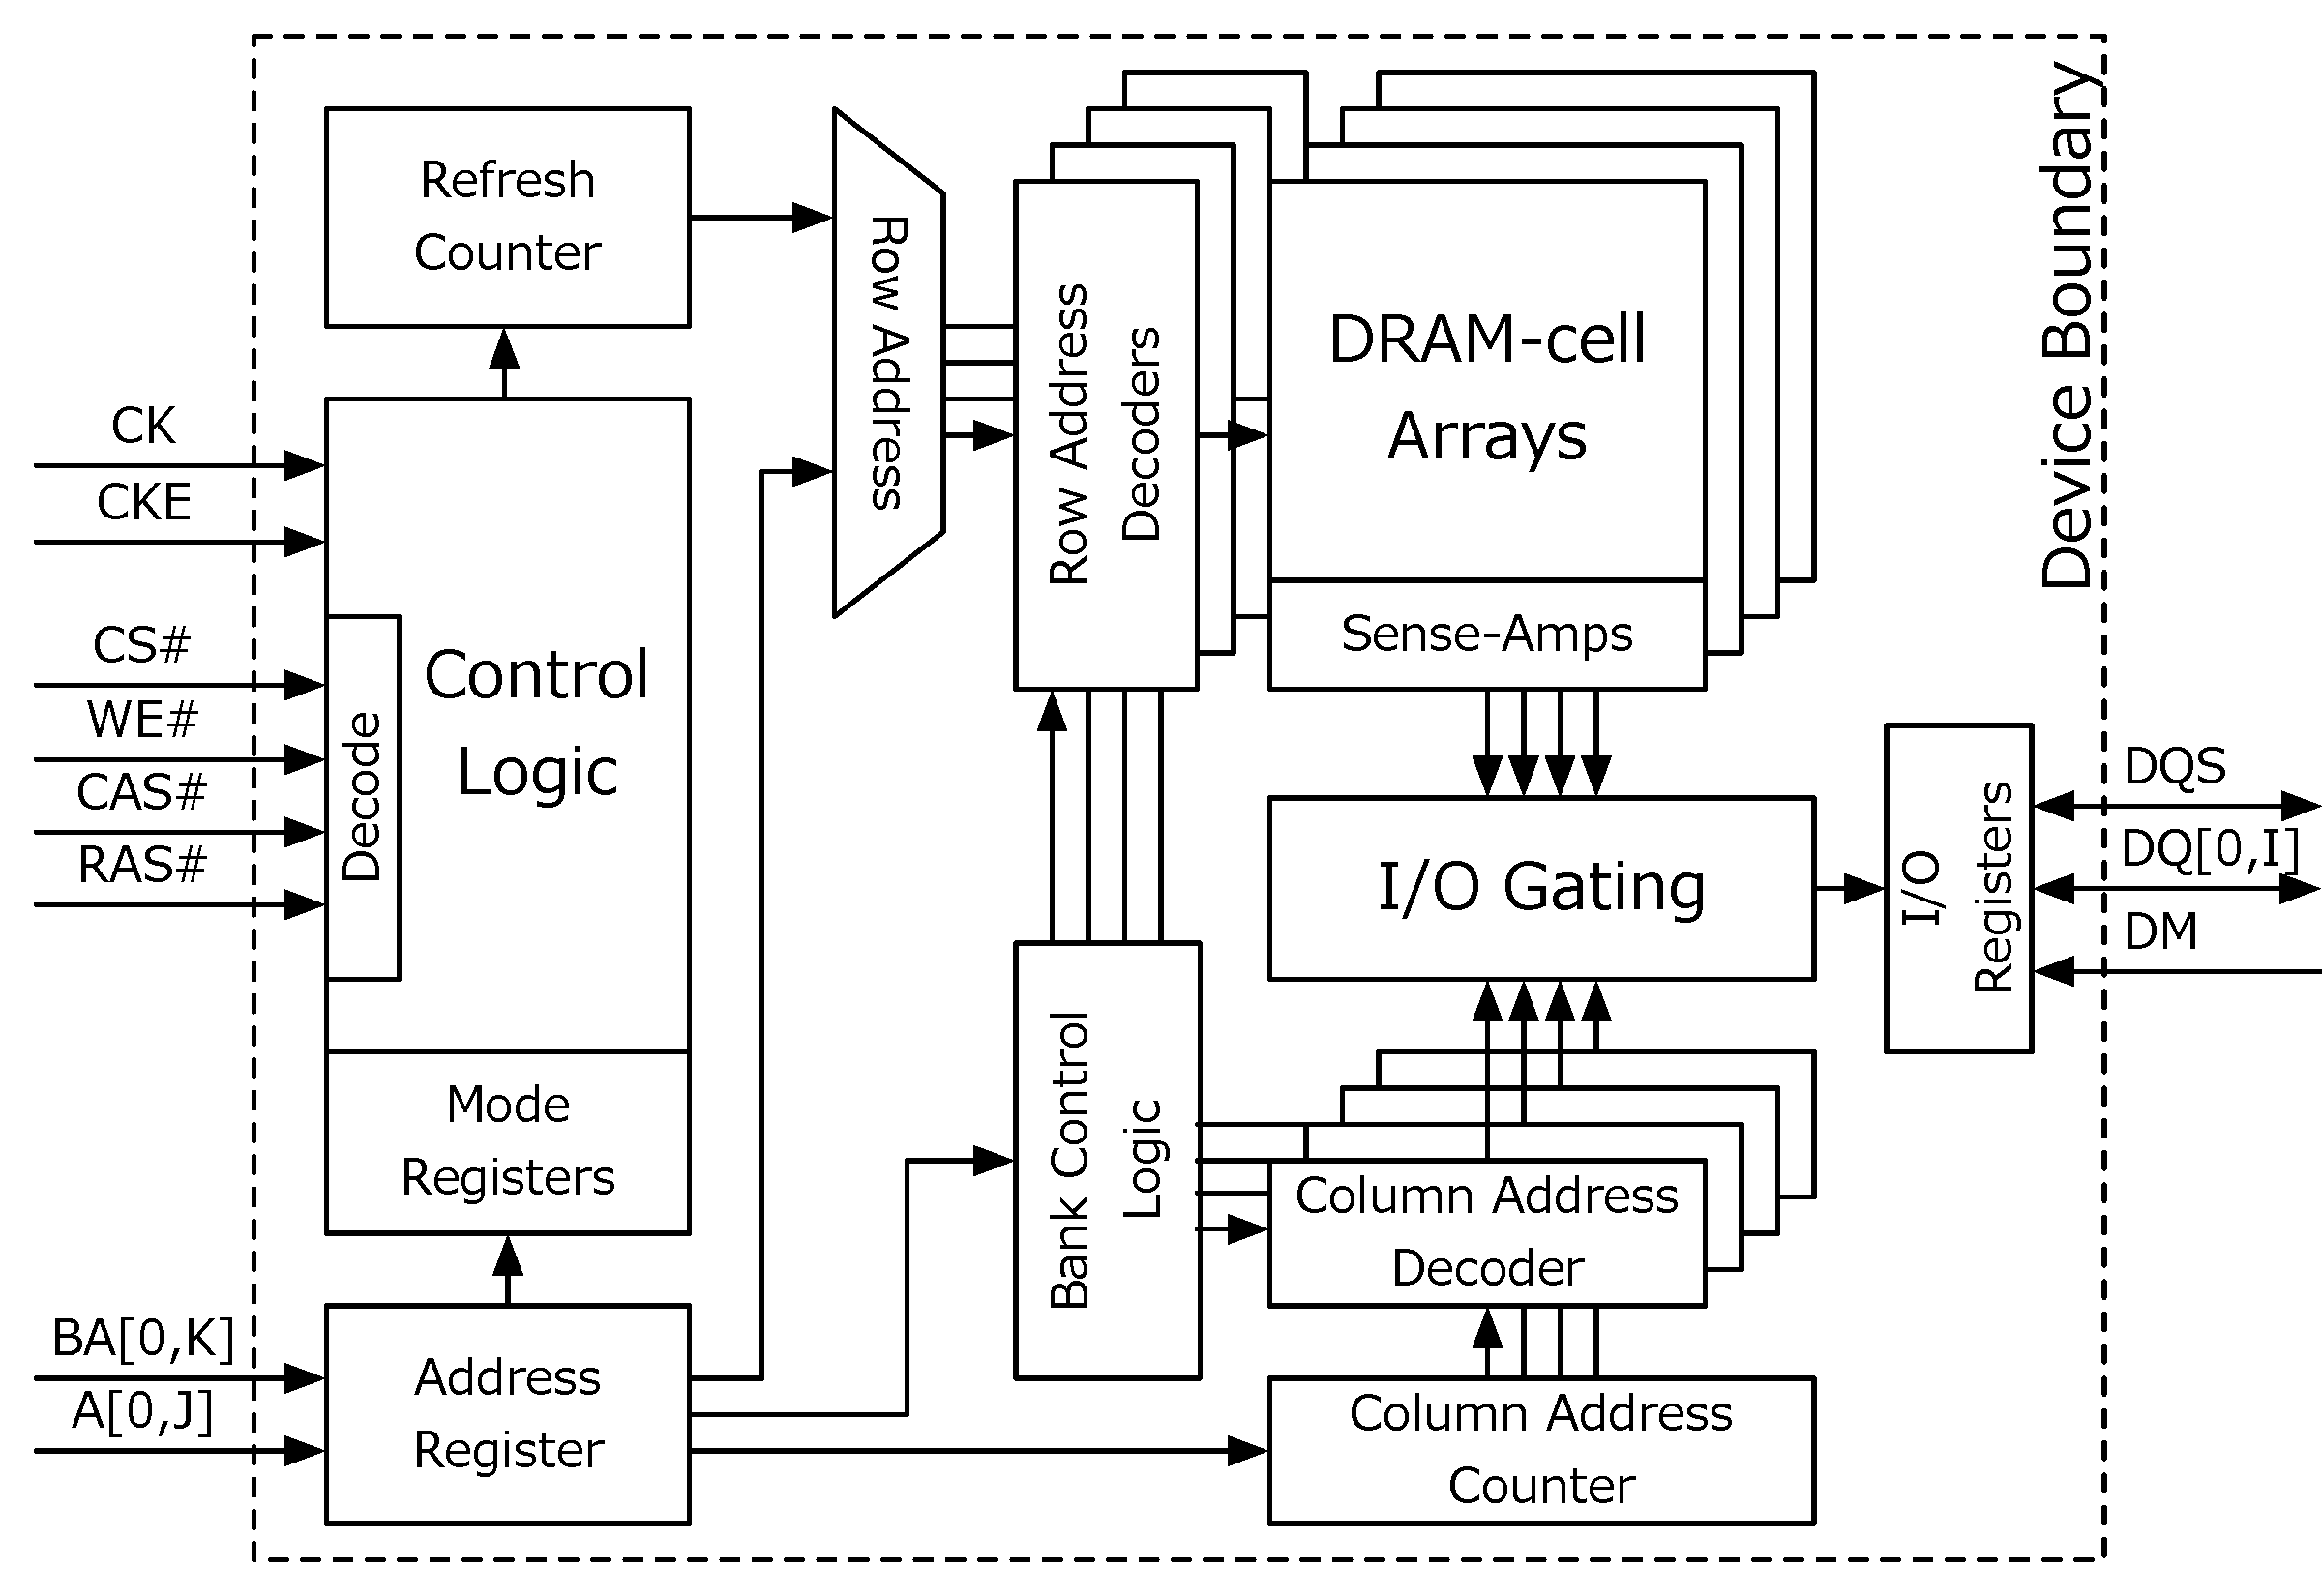
\includegraphics[width=\columnwidth]{figures/dram-device.pdf}
%     % graffle2pdf -c device midas-graphics/graffle/dram-diagrams.graffle figures/dram-device.pdf
%    \caption{The organization of a typical DRAM device.}
%	\label{fig:dram-device}
%\vspace{-0.12in}
%\end{figure}

DRAM gradually loses its stored state over time as bit cell capacitors leak. To
maintain their state, DRAM cells must be periodically refreshed. In the DDR
standards, JEDEC mandates that cells must be refreshed once every 64
ms. Since activations to every row cannot generally be guaranteed during normal
use, DRAM devices are refreshed explicitly with a refresh command~(REF). To
reduce complexity, this command refreshes a constant number of contiguous rows
in all banks concurrently. DRAM manufacturers generally have kept the number of
refresh commands required to iterate through the entire array constant: 8192
commands per 64 ms interval, or one every 7.8 $\mu s$.
% is there a citation for this ^
\section{DRAM Controller Architecture}\label{sec:dram-mas}
A DRAM controller is responsible for responding to memory
requests from one or more requesters by scheduling those requests over its
memories as a judicious stream of DRAM commands.

Memory access scheduling~(MAS) is the process by which, for a given cycle, a
controller selects a single DRAM command to be issued from a legal set. Legal
commands are constrained by the current state of each bank, the availability of
shared resources like the command and data buses, and timing constraints
imposed by the DRAM devices. Good MAS policies strike a balance
between minimizing latency, maximizing bandwidth, minimizing power, and
maintaining quality-of-service guarantees. In this paper we consider two common
MAS policies: First-Come First-Served~(FCFS) and First-Ready
FCFS~(FR-FCFS)~\cite{frfcfs}.

In a FCFS MAS, commands for the oldest pending memory reference are issued
first. This is the simplest MAS policy, but tends to under-utilize available
DRAM bandwidth as younger requests that may hit an open row buffer must wait
behind commands that miss. In a FR-FCFS MAS, first, ready~(legally issuable) column
commands are prioritized over ready row commands. Second, commands for older
references are prioritized over younger ones. This permits younger but ready
column commands to be issued before older row commands, improving DRAM bandwidth
utilization considerably.

%\section{Power Consumption in DRAM Memories}\label{sec:dram-power}
%
%DRAM power consumption can be divided into six different classes: activation
%(including precharge), read, write, termination, refresh, and background power.
%
%Activation is generally the largest component of DRAM power consumption.  In an
%effort to maximize areal density and reduce cost-per-bit, DRAM sub-arrays have
%long, high capacitance bitlines, which are driven to VDD or ground during the
%restore phase of an activation. Moreover, DRAM rows are long: thousands of
%bitlines are simultaenously charged or discharged in a single activation. These
%two properties lead to high peak-current draw during an activation. In order to
%stay within a power envelope where DRAM devices can be cooled passively without
%heatsinks, DRAM manufacturers put limits on activation frequency through
%$t_{RRD}$ and $t_{FAW}$ constraints (see table\ref{tbl:dram-timings}).
%
%Read and write power consumption accounts for the power dissipated as data is
%driven between the I/Os of the chip and its various sub-arrays, as well as the
%power used to decode the read or write command.
%
%Refresh power accounts for the power lost during the successive activations and
%precharges of a refresh command. It is a growing component of power consumption
%as modern DRAM devices trend towards higher row counts. Higher row counts impose
%that more rows must be refreshed per command which forces the device to spend
%more time in refresh (higher $t_{RFC}$).
%
%Termination power accounts for the power dissipated in on-die termination
%resistors of a device during a write, and by the output buffers of a device
%during a read. In multi-rank systems, this also includes power dissipated in
%the termination resistors of ranks not being addressed.
%
%Finally, background power accounts for leakage of various circuits within the
%IC. Here there are two dimensions of note. First, activated banks
%leak more than precharged banks. Second, powered-down ranks~(CKE low) leak less
%than powered-up ranks~(CKE high).


\section{DRAM Memory System Simulators}

The current state of the art in DRAM simulation in academia is cycle-accurate
software simulators like~\cite{dramsim, ramulator, usimm}. These simulators
generate DRAM command streams that have been validated against industrial
models. In trace-driven mode, operating at full throughput and only as a
timing-model, these models simulate at rates of
hundreds of KHz to ones of MHz~(reported in \cite{ramulator}).
%
%To model power dissipation, Micron white papers~\cite{micronpower} describe a strategy that
%assigns an average current draw to different modes of power dissipation. Micron
%has encoded this in freely available spreadsheets that generate estimates based
%on system-level measurements of DRAM activity, such as row-buffer hit rate.
%DRAMSim2 directly implements the Micron approach by integrating the appropriate
%current based on the state of the memory system.

%One limitation of the Micron approach, is that it does not account for the
%power dissipation of the controller itself. However, for modest memory
%controller implementations, this should be small.

% OLD DRAM Section
%We will now review important first-order architectural
%characteristics of DRAM memory-systems that we model in our initial set of
%timing models.
%
%\subsection{DRAM Device Architecture and Organization}
%
%In a DRAM IC, arrays of bit cells are hierarchically arranged into multiple
%parallel \textit{banks}. Banks provide the primitive level of concurrency in a
%DRAM memory system. They can service independent requests, assuming they do not
%simultaneously require shared resources like the data, address and command
%buses.  Multiple DRAM ICs can be arranged in parallel to widen the data bus;
%address and command buses fan out to each IC.
%
%A basic DRAM operation requires a series of three commands: \textit{activate (ACT)},
%\textit{column access (CAS)}, and \textit{precharge (PRE)}. The ACT command enables the word-lines of the array corresponding to a single \textit{row} of the bank. The cells of the row are
%sensed and saved in a \textit{row buffer}(typically O(1) kB). A CAS command then selects a subset
%of the row buffer to read or write; data is bursted over successive clock edges. While the row
%buffer remains \textit{open}, the row can be accessed by issuing new CAS commands. To access a
%row not stored in the buffer, a PRE command must be issued to \textit{close} the row and charge
%the bit-lines for a new access.
%
%\subsection{DRAM Controller Architecture}
%
%At the highest level, a DRAM controller is responsible for responding to memory
%requests from one or more requestors by scheduling those requests over its
%attached memories as a judicious stream of DRAM commands.
%
%Memory access scheduling (MAS) is the process by which, for a given cycle, a
%controller selects a single DRAM command to be issued from a legal set. Legal
%commands are constrained by the current state of each bank, the availability
%of shared resources like the command and data buses, and timing constraints
%imposed by the DRAM standard. Good MAS policies strike a delicate balance
%between minimizing latency, maintaining quality-of-service guarantees across
%multiple threads of execution, maximizing bandwidth, and minimizing power.
%There are plethora of academic papers on MAS policies, and still more
%industrial patents on the subject. We outline some of the most popular MAS policies
%here.
%
%\subsection{First-Come First-Serve (FCFS) Policy}\label{fcfs}
%Commands for the oldest pending memory reference are always issued first. This
%is the simplest MAS policy, but one that grossly under-utilizes available DRAM
%bandwidth. FCFS schedulers are common in older machines, and those that present
%few concurrent memory requests.
%
%\subsection{First-Ready FCFS (FR-FCFS)\cite{frfcfs} Policy}\label{frfcfs}
%First, column access commands that hit in an open row-buffer are prioritized,
%then row and precharge commands from the oldest pending reference are
%considered.  FR-FCFS is a relatively simple scheme that achieves far higher BW
%than FCFS. It is the de facto standard against which new MAS policies for
%machines with a single stream of memory references (like single-core
%out-of-order machines), are compared.
%
%\subsection{DRAM Software Simulation}
%
%The current state of the art in DRAM simulation in academia are cycle-accurate
%software simulators like DRAMSim2\cite{dramsim}, Ramulator\cite{ramulator} and
%USIMM\cite{usimm}. These models generate DRAM command streams that
%have been validated against industrial models (for some standards). Both
%Ramulator and DRAMSim2 can be easily integrated into Gem5\cite{gem5}, though it
%includes a detailed event-based model of its own\cite{gem5event}. In trace-driven mode, operating at full throughput and only as a timing model, these
%cycle-accurate models simulate at frequencies ranging from 100s of KHz to ones
%of MHz\cite{ramulator}.

%\subsection{DRAM Power Modeling}

%In order to model power, Ramulator relies on DRAMPower\cite{drampower}, to which it passes its command trace. Micron describes strategies in their technical notes for estimating DRAM power\cite{micronpower} (which DRAMSim2 employs). They also made these calculations accessible by providing spreadsheets that take micro-architectural event frequencies as input. These approaches can carry over to FPGA simulation, as sufficiently detailed FPGA models can add instrumentation for these events, while simpler models can save the memory access trace to a buffer and compute power out-of-band\cite{strober}.
